%*******************************************************
% Background
%*******************************************************

\chapter{Background and Literature Review}
\par In this chapter we will provide contextual information on the issue of fossil fuel dependence as well as the application of renewable energy sources in public buildings in the U.S. This chapter also includes an explanation and comparison of different renewable energy types to provide background on existing and emerging technologies for thermal heating and cooling and their respective advantages. Additionally, information on how the Commonwealth's energy resources and regulations factor into the success of the DOER's renewable thermal project sites is provided.

  \section {Fossil Fuel Dependence and its Consequences}
  \par The United States has depended on non-renewable resources as a source of power since the 1800's when oil and coal were discovered to be more energy dense than wood (Samimi, \& Zarinabadi, 2012, WaitButWhy, 2015). Figure \ref{fig:pie} represents the percentages of the total energy consumed in the United States. More than 80\% of the total energy consumed by the country comes from a non-renewable source of energy (U.S. Energy Information Administration, 2015).
  \begin{figure}[h]
    \centering
      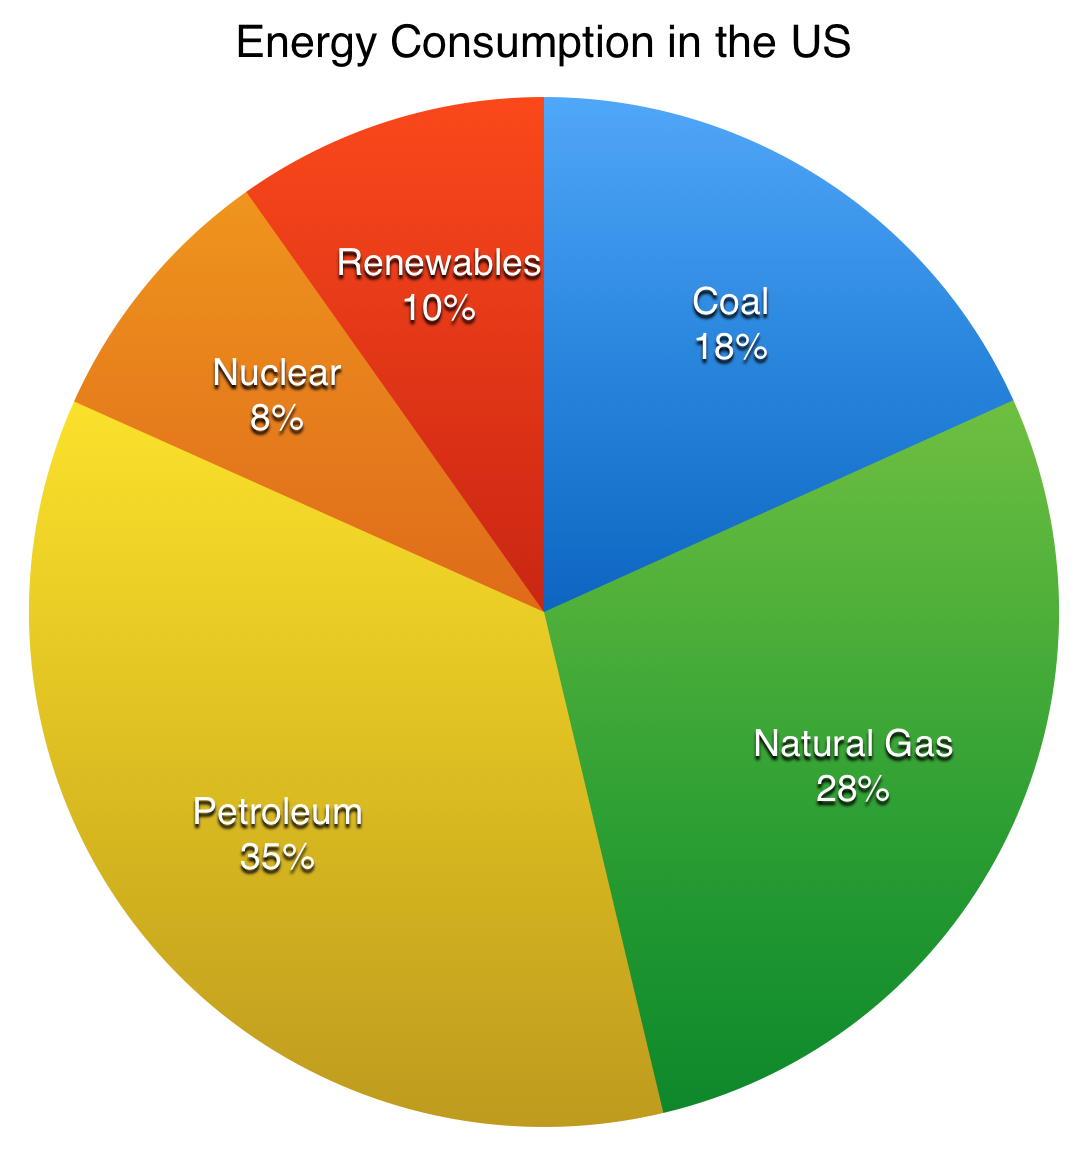
\includegraphics[width=0.70\textwidth]{images/01-EnergyConsuptionPieChart}
    \caption{Energy Consumption in the US (U.S. Energy Information Administration, 2015)}
    \label{fig:pie}
  \end{figure}
  \par These sources are limited and are damaging to public health and the environment. The use of fossil fuels is a threat to public health due to the effects that greenhouse gas emissions and other pollutants can have (Haines, Kovats, Campbell-Lendrum, \& Corvalán, 2006).  The pollution caused by fossil fuels is directly related to health problems such as asthma, ischemic heart disease, chronic bronchitis, cancers, and increasing mortality rate, among others (Rabl \& Spadaro, 2000; Kampa, \& Castanas, 2008). The use of fossil fuels is responsible for 76\% of the total greenhouse gas emissions released by the United States. Greenhouse gases create a layer around the Earth that keeps solar radiation within the atmosphere in order to keep the Earth's average temperature suitable for life (Samimi, \& Zarinabadi, 2012).  As the concentration of greenhouse gasses in the atmosphere grows however, it will keep more solar radiation and warmth inside the atmosphere, elevating the average temperature of the Earth (Samimi, \& Zarinabadi, 2012). This temperature change can lead to catastrophic climate changes in the world such as the melting of the ice poles, sea level rise, and others (U.S. National Climate Assessment, 2014).
  \par Greenhouse gasses are not the only detriment from the pollution that burning fossil fuels produces. Acid rain is directly linked to fossil fuels due to the sulfur dioxide and nitrogen oxides that power plants release when burning fossil fuels (U.S. Environmental Protection Agency, 2012). Acid rain can negatively affect the biodiversity of our planet by changing the pH of water and acidifying soils (Likens, 2011). A recent survey in the Northeast of the United States showed that 41\% of lakes in the Adirondack Mountain region are acidic or subject to short-term pulses in acidity related to snowmelt and rain storms. Similarly, the same characteristics were found in 15\% of the lakes in the areas of Catskill and New England (Likens, 2011).
  \par Fossil fuels also damage the environment through accidents and industrial extraction processes such as oil spillages and fracking. Oil spillages affect a great variety of animals, both in the ocean and in surrounding areas (Office of Response and Restoration, 2015). Light oils such as gasoline or diesel are highly explosive and toxic therefore they can kill animals and plants that they touch and can also affect human beings who inhale the fumes. Heavy oils are black and sticky substances commonly used to fuel ships. In the short term these oils can cover organisms affecting their mobility and can also affect their ability to keep warm; many birds die from hypothermia due to these oil spillages (Office of Response and Restoration, 2015). In the long run, exposure to heavy oils might result in health problems such as tumors in organisms (Office of Response and Restoration, 2015). Fracking is a natural gas harvesting process that uses and contaminates large quantities of water. In fact, annual water consumption by fracking is equivalent to the annual water consumption of 40 to 80 cities with populations of 50,000 each (Gold, 2014). Figure \ref{fig:power} illustrates how natural gas use in Massachusetts has grown while coal and oil use have declined. This growth results in increased fracking to keep up with the increasing demand for natural gas.
  \begin{figure}[h]
    \centering
      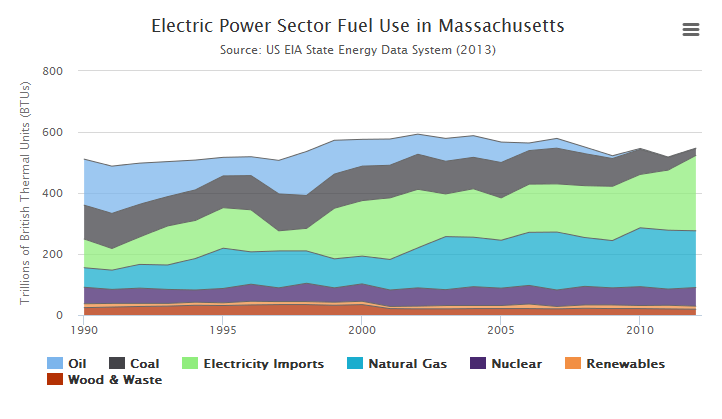
\includegraphics[width=\textwidth]{images/02-ElectricPowerSectorFuelUseinMassachusetts}
    \caption{Electric Power Sector Fuel Use in Massachusetts (EIA, 2013)}
    \label{fig:power}
  \end{figure}
  \par The use of fossil fuels is damaging the world in multiple ways, and as the world needs more energy, the pollutants derived from the use of fossil fuels increase. The U.S. Energy Information Administration has projected that the world's energy consumption will increase by 56\% by 2040 (Samimi, \& Zarinabadi, 2012). Increasingly, buildings are becoming a large portion of this energy consumption and are thus an area for concern (Rezaie, 2013).

  \section{Energy Use of the Buildings Sector}
  \par Buildings contribute greatly to our greenhouse gas emissions. In developed countries, 50\% of the CO\textsubscript{2} emissions and 40\% of the energy consumption can be attributed to buildings (Rezaie, 2013). Because of the development of more buildings and their increased energy use, buildings are now the largest sector of energy use, drawing more than the transportation and industrial sectors in most developed countries (EIA, 2015). The United States is one of the countries with the highest building energy use, consuming 41\% of the country's total energy, while the EU and the rest of the world use less energy in buildings at 37\% and 24\% respectively (EIA, 2014; Perez-Lombard, 2008). 
  \par There are many factors contributing to the increased energy use in buildings within industrialized nations. Use of computers and other office equipment drives up the electricity consumption along with lighting, heating, and cooling (Spyropoulos, 2011). As people spend more and more time inside, working, taking classes, etc., the cost of powering those buildings increases (Perez-Lombard, 2008). Office buildings particularly, running mainframes and powering computers for all employees, are drawing increasingly more power (Eichholtz, 2010). Energy consumption due to lighting has also gone up in recent years, although this consumption is predicted to decrease in the near future because of the expected adoption of efficient Compact Fluorescent Lamps (CFLs) and LED lighting with sophisticated controls (Spyropoulos, 2011).
  \par Heating and cooling are large energy draws in most buildings and are becoming more necessary with the amount of time people have been spending indoors. In an energy audit of school buildings in Italy, thermal consumption was 80\% of the energy consumed (Desideri, 2002). This is not uncommon: in the average Massachusetts household, thermal energy use represents about 75\% of the energy consumption with space heating the biggest component (60\%) (EIA, 2015).
  \par With buildings using large amounts of energy, especially for heating and cooling, many alternative energy options have been researched to decrease the greenhouse gas emissions from energy use and buildings. Data from one case study in Ontario, presented in Table \ref{tab:energyuse}, shows the distribution of different draws of energy in a typical residential building as well as common sources of energy for them. The rightmost column in Table \ref{tab:energyuse} shows possible alternative energy sources that can improve the energy efficiency of the building. Appliances, lighting, and “other” can use electricity generated on site by any solar, wind, or other renewable sources.
  \begin{center}
    \begin{table}[h]
      \caption{Energy Use in a Residential Building Energy Use in a Residential Building (Rezaie, 2013)}
      \begin{adjustwidth}{-0.5in}{-0.5in}
        \centering
          \begin{tabular}{|p{1.25in}|p{1in}|p{1.5in}|p{1.75in}|}
            \hline
            \thead{Energy Draw} & \thead{Amount of Energy} & \thead{Common Sources} & \thead{Alternate Technologies} \\ \hline
            Space heating and cooling & ~ 55\% & Heating oil, coal, propane, electricity, natural gas & Biomass, solar thermal, geothermal, air \& water source heat pumps \\ \hline
            Hot water heating & ~ 20\% & Heating oil, coal, propane, electricity, natural gas & Solar thermal, biomass, heat pumps \\ \hline
            Lighting & ~ 5\% & Electricity generated at power plants using natural gas, coal, or nuclear & Electricity generated by wind, solar, photovoltaic, wood, geothermal for electricity generation \\ \hline
            Appliances & ~ 15\% & Electricity generated at power plants using natural gas, coal, or nuclear & Electricity generated by wind, solar, photovoltaic, wood, geothermal for electricity generation \\ \hline
            Other & ~ 5\% & Electricity generated at power plants using natural gas, coal, or nuclear & Electricity generated by wind, solar, photovoltaic, wood, geothermal for electricity generation \\
            \hline
          \end{tabular}
      \end{adjustwidth}
      \label{tab:energyuse}
    \end{table}
  \end{center}
  \par HVAC systems are the largest draw of energy in buildings, pulling on average 50\% of a building's energy (Perez-Lombard, 2008). The energy use in buildings by heating and cooling systems will continue to increase as industrialized nations build more and bigger buildings, although improvements in energy efficiency and smarter building design may be able to mitigate this increase in heating and cooling energy use (Perez-Lombard, 2008). Additionally, older buildings with very low energy efficiency use much more energy in heating and cooling than they otherwise would if newer technologies were used in the buildings (Krawcyzk, 2014). With HVAC being the largest sector of energy use within buildings, which is the largest sector of energy consumption in the developed world, it's clear that heating and cooling in buildings is a huge target for improvement.

  \section{Transitioning Between Fossil Fuels and Renewable Energy}
  \par One of the potential solutions to the problem of fossil fuel dependence and the harm they have on the environment and public health is the use of renewable energy. The Oxford Dictionary defines renewable energy as energy from a source that is not depleted when used. With a growing population and increase in energy demand, the use of renewable energy is intended to promote a sustainable future without large adverse effects on the environment (Samimi, \& Zarinabadi, 2012). The transition from fossil fuels to renewables is certainly a complex process requiring the involvement and consideration of many groups and factors. Some of the aspects that impact this transition from fossil fuels to renewable resources include public opinion, overall cost, any kind of performance metering that may be desired or required, and potential obstacles (EEA, 2015).

    \subsection{Public Opinion on Renewable Energy Systems}
    \par When implementing a public project with renewable energy, the sponsor needs to take into consideration the public's view of the project. If the project is not socially accepted, it has a higher likelihood of failing. If the public accepts the program, sponsors like the Department of Energy Resources (DOER) will be able to provide grant money and expand the reach of their renewable energy programs.
    \par One reason why the public might not accept the implementation of renewable heating and cooling systems in buildings is the uncertainty as to whether or not renewables are able to maintain climate control as well as current energy sources. The reason for this is twofold: people are often unaware of how these new technologies work because of how recently they have been brought to the energy market, and even if they are familiar with the technologies they often do not trust the systems until they've seen them in use themselves (Karlstrom, Ryghaug, 2014).
    \par Consequently, potential project leaders can change the negative assumptions the public in their community has about renewable technologies by removing the “knowledge deficit” (Brunk, 2006). This deficit in knowledge could be reduced by education or persuasive communication, where the sponsor can help the public understand that renewable technologies not only perform as well as current energy resources, but also reduce greenhouse gas emissions and do not harm our environment (Brunk, 2006). Studies have shown that the public support for renewable resources increases if they are given thorough information about the pros and cons of the implementation of these technologies (Ogarra, Mourato, and Pearson 2005). The community understanding and supporting the technology does not guarantee that the project will succeed though. They may support the technology, but not the way it's proposed to be implemented, or the cost or timing of the project. But with community support for the technology, the details of the project can then be worked out to maximize support for the project.
    \par Public opinions tend to become more positive once a project is implemented and people understand the economic benefits (Karlstrom, Ryghaug, 2014). One way to address the knowledge deficit after project implementation is through educational programs, such as kiosks at the location of the project or webpages. The Ferrisburgh Solar Farm, which was built in Vermont, is a 3,806 solar panel system, installed by REV Corporate Member Alteris Renewables (Renewable Energy Success Stories, 2015). After the implementation of this project, the Solar Farm created an open-to-the-public educational kiosk where they provide the information about the benefits of the project. They also published a website on the internet that tracks the solar energy output of their farm (Renewable Energy Success Stories, 2015). If the public comes to understand how renewable technologies work, they may begin to support more renewable energy projects, which would aid in their community's transition away from fossil fuels and toward renewable energy sources.

    \subsection{Cost and Pricing of Renewable Energy Systems}
    \par Making the choice to switch to renewable resources is just like many other long term investments. The upfront cost is high, but in the long term, it will save money. For example: buying a car is a long term investment where generally the longer you keep the car, the more value you get out of the investment, but if you only look at the short term, leasing may be more cost effective. Installing renewable energy sources can pose a large upfront cost, but some renewable resources have lower operating costs than fossil fuels and thus will save money in the long term (BEAM Engineering, 2014; D.C. Architects, 2014; DOER, 2015; RDK Engineers, 2014; Wilson Engineering, 2015). In order to lighten the load of the upfront initial cost, there are many government funds allocated to help renewable energy projects. Despite the effort toward incentivizing renewable energy projects, the World Bank and International Energy Agency put global annual subsidies for fossil fuels in the range of \$100 billion to \$200 billion, making renewable energy programs appear even more expensive by comparison (Beck \& Martinot, 2004).
    \par Many different costs factor into the high upfront cost of installing a renewable thermal technology. The assessing of the property, permitting, and planning add to the upfront cost, as they must be completed by a contracted, qualified, and well-experienced engineering firm (DOER, 2015). These renovations can completely change a building's heating and cooling system, which is an expensive change as well (Beck \& Martinot, 2004). After all the support work, the actual renewable energy technologies need to be purchased, and they may face high taxes and import duties (Beck \& Martinot, 2004). Where renewable energy technologies excel, however, is in the operations and fuel costs, where many renewable resources, such as solar, don't need to pay for fuel at all. Additionally, once the system is operational, the maintenance costs of the systems are often similar to the costs associated with fossil fuel heating systems (BEAM Engineering, 2014; Wilson Engineering, 2015).

    \subsection{Performance Metering in Renewable Energy Systems}
    \par When considering the implementation of a renewable thermal project, multiple stakeholders are interested in knowing a tangible amount of cost savings that they can expect to see (Massachusetts Department of Energy Resources, 2015). Additionally, once a project has been completed many owners want to know exactly how much money they are saving with their new installation. The way to obtain this information is generally through performance metering technology. There are multiple types of performance metering ranging from just looking at total energy consumption per month, to monitoring each circuit in the building on a minute by minute basis.
    \par The Department of Energy Resources uses two metering systems for the installations that they fund: Mass Energy Insight and Energy Star Portfolio Manager. These both just look at the monthly power consumption, so there is not very detailed data on power usage. PowerWise is a metering tool that the DOER has begun working with in order to close this gap. PowerWise consists of hardware installed inside the electrical panels that communicates to an online interface. This interface shows information relating to electricity use for each major appliance including energy use and cost for varying time intervals (i.e. monthly, weekly, daily) (DOER, 2015). For more information on PowerWise, see Appendix 1.

    \subsection{Potential Obstacles in Transitioning to Renewable Energy Sources}
    \par In any renovation, there are multiple potential obstacles to be aware of. Many renewable energy programs focus on projects in buildings where the fossil fuel systems are in disrepair or need be replaced. Rather than simply replacing an oil boiler, for example, a renewable energy project may require the implementation of a completely new heating and cooling system. With a renovation this large, there are many problems that can be encountered, including but not limited to: old electrical systems, asbestos, and lead paint. These could cause logistical delays and can also result in a more complex and expensive renovation (Massachusetts Department of Energy Resources, 2015).
    \par In addition, renewable systems such as wind turbines, rooftop solar hot-water heaters, photovoltaic installations, and biomass combustion systems may face restrictions based on parameters such as height, noise, and aesthetic concerns. These restrictions vary based on the implementation site, so extensive background research is required before starting a renewable energy project (Beck \& Martinot, 2004).

  \section{Massachusetts and Energy Efficiency/Renewable Energy Programs}
  \par Despite the difficult process of transitioning to renewable energy systems, Massachusetts is committed to increasing the use of renewable resources to decrease greenhouse gas emissions. Focusing on buildings with regards to energy is especially important for Massachusetts because buildings account for 49\% of all energy consumed in the Commonwealth, compared to 41\% nationally (EIA, 2015). Ranked 5th with the most LEED certified buildings in the United States, the Commonwealth of Massachusetts has become a leader in energy efficiency and alternative/renewable energy use (USGBC, 2015). This success in LEED certifications is due in part to the many supportive energy efficiency and renewable energy grants, programs, and regulations in the Commonwealth of Massachusetts. An important part of Massachusetts' efforts to promote the use of renewable energy resources is the Green Communities Act of 2008.
  \par The Green Communities Act prompted programs to boost energy efficiency and encourage investment in renewable energy (Conservation Law Foundation, 2010). This act also requires utilities to increase investment in energy efficiency, reducing demand and delivering savings to customers. The Green Communities Act mandates the design and implementation of three year energy efficiency plans for gas and electric utilities, provides funding for energy efficiency projects, and requires that 15\% of all electricity be supplied by new renewable power facilities by 2020  (Conservation Law Foundation, 2010).
  \par With the Green Communities Act of 2008 legislation in place, funding and guidelines became available for emerging energy efficiency and renewable energy programs to utilize. As a result, many programs within Massachusetts aim to further the Commonwealth's energy efficiency and renewable energy successes. The Massachusetts Clean Energy Center (Mass CEC) is an agency that was developed in 2009, immediately following the Green Communities Act. The Mass CEC  is dedicated to accelerating the success of clean energy technology through providing funding for renewable energy rebates for residents and businesses (Mass CEC, 2015). Another important program for the progression of energy efficiency and renewable resources is the Massachusetts School Building Authority (MSBA). The MSBA has started sustainable programs with emphasis on reducing energy and water consumption (MSBA, 2011). The MSBA also utilizes the MA Collaborative point system to assess potential projects in high performance schools and how much, if any, funding they will provide to aid these projects (MSBA, 2011). This Green Schools program under the MSBA pays a percentage of the total cost to renovate schools that wish to increase energy efficiency and/or install a renewable energy heating and cooling system (MSBA, 2011).

    \subsection{Specific Energy Efficiency/Renewable Energy Programs in Buildings}
    \par There are many building focused energy programs within the Commonwealth of Massachusetts. For example, the \emph{Building America: Bringing Buildings Innovations to Market}  program focuses on improving building energy performance in residences all over the country; however, it has a concentrated focus on the Commonwealth of Massachusetts due to the Commonwealth's energy programs and legislation (EERE, 2015). Another similar program with large focus in Massachusetts is \emph{Better Building Partners}, a program that works with communities to promote energy efficiency in homes and other buildings. In order to achieve these goals, the program works with city and statewide partners (EERE, 2015).

    \subsection{DOER's Renewable Thermal Programs}
    \par Among the different programs for the implementation of renewable resources offered in Massachusetts are the focuses of our project: the DOER's Renewable Thermal Program and the Schools and Public Housing Integrating Renewables Efficiency (SAPHIRE) program. The goal of these DOER programs is to help municipalities, schools, and public housing initiatives install renewable heating and cooling systems across the Commonwealth (Massachusetts Department of Energy Resources, 2015). The programs have been successful so far in beginning to reach their goals of implementing renewable thermal heating and cooling systems in different types of buildings. 
    \par The DOER's Renewable Thermal Program and SAPHIRE program focus mainly on public buildings for several reasons. The first is that the programs are using government funding, so it makes logical sense to use these resources to improve public resources and decrease the expenses of public facilities. The second reason is that public buildings require a lot of energy: 49\% of all energy in Massachusetts. Public buildings are often relatively large in size, and thus consume a lot of energy for heating and cooling. Also, even if individuals change their residences to use renewable energy for heating and cooling, a community won't be completely sustainable until the public resources are addressed, which is the responsibility of the government (Office of Energy Efficiency and Renewable Energy, 2015).

  \section{Renewable Energy Technologies}
  \par Renewable energy comes in many different packages. There are multiple renewable sources of energy in the market used to generate either electricity (measured in kilowatt hours (kWh)) or heating energy (measured in British Thermal Units (BTUs)). With the relatively high consumption of BTUs in buildings in the Northeast, the DOER has developed incentive programs to support renewable sources of heating and cooling: solar thermal, geothermal, biomass and most recently, air source heat pumps. In this section, we will provide a description of each renewable energy technology as well as its advantages and disadvantages. Since the scope of our project is within Massachusetts, we will provide relevant information on these technologies with regards to their application in the Commonwealth of Massachusetts. 

    \subsection{Solar Thermal}
    \par A solar thermal system consists of panels that absorb the energy of the sun to heat pipes with water (or another liquid) that then will heat the building spaces or provide hot water heating (as seen in Figure \ref{fig:solar}) (Massachusetts Department of Energy Resources, 2015).
    \begin{figure}[h]
      \centering
        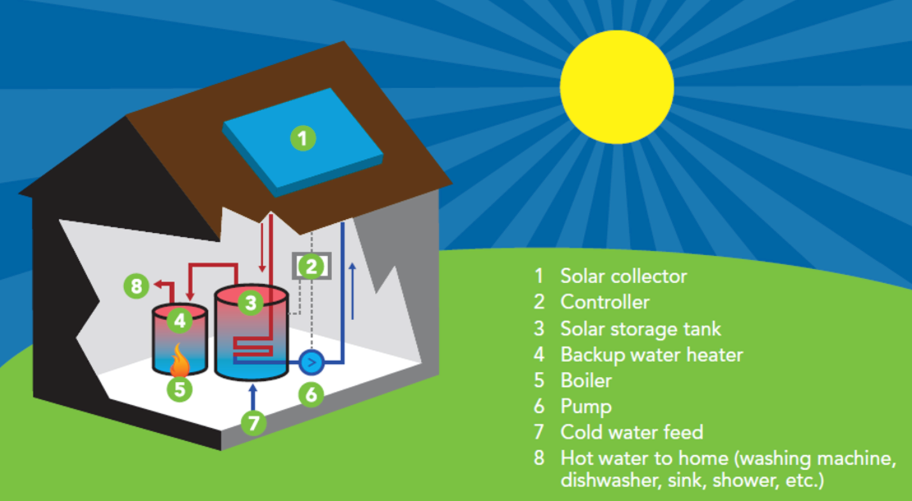
\includegraphics[width=0.75\textwidth]{images/03-SolarHotWaterHeatingSystem}
      \caption{Solar Hot Water Heating System (Massachusetts DOER, 2015)}
      \label{fig:solar}
    \end{figure}
    \par Solar thermal systems differ from solar photovoltaic (PV) systems in that they generate thermal energy instead of electricity. Solar thermal systems have multiple advantages and disadvantages related to the use and installation, which are important to consider in order to understand when and where this solar thermal system might be applicable and efficient. Below we provide a summary of the advantages and disadvantages of using a solar thermal system.\\

    \vbox{
    \noindent
    Advantages of a Solar Thermal System:
    \begin{itemize}
      \item{Used to heat liquids such as water that then can be used for showers, pools and laundry (Massachusetts Department of Energy Resources, 2015).}
      \item{Can also be installed in such way that it will integrate with the HVAC system and provide space heating. (Massachusetts Department of Energy Resources, 2015).}
      \item{Using solar panels, this system can often provide between 50-75\% of the total building's hot water needs (depending on roof exposure, weather, and system size) (Massachusetts Department of Energy Resources, 2015).}
      \item{Able to store energy for when the sun sets and is able to provide some energy during cloudy days (Massachusetts Department of Energy Resources, 2015).}
      \item{Incentives can save customers up to 50\% of the cost of the system, through the Commonwealth Solar Hot Water Rebate program, and 0\% interest HEAT loans are also available through Mass SAVE (Massachusetts Department of Energy Resources, 2015).}
    \end{itemize}
    }
    \vbox{
    \noindent
    Disadvantages of a Solar Thermal System:
    \begin{itemize}
      \item{Solar panels can be expensive and intermittent; therefore, they can't be used as the only source of power to meet the base load energy demand of a building (Massachusetts Department of Energy Resources, 2015).}
      \item{Depending on the quality of the solar panels they might actually emit some greenhouse gases such as nitrogen trifluroide and sulfur hexafluoride (Maehlum, M. A., 2014)}
    \end{itemize}
    }

    \subsection{Geothermal Heating and Cooling}
    \par A geothermal system consists of pipes placed around 300-900 feet underground that carry water via either a closed-loop or open-loop configuration (Massachusetts Department of Energy Resources, 2015). The water absorbs the underground heat present, as the temperature under the surface of the Earth is a relatively consistent 50 degrees Fahrenheit (Massachusetts Department of Energy Resources, 2015). This process can be reversed in the summer. Indoor heat is extracted from the building and transferred to the earth through the liquid (Massachusetts Department of Energy Resources, 2015). Geothermal heat pumps are 3.5 - 5 times as efficient as the most efficient fossil fuel furnace. Instead of burning a combustible fuel to make heat, they simply move heat that already exists. By doing so, they provide 3.5 - 5 units of energy for every unit used to power the heat-pump system (Massachusetts Department of Energy Resources, 2015). Figure \ref{fig:geo} is a graphic representation of how a geothermal system operates.
    \begin{figure}[h]
      \centering
        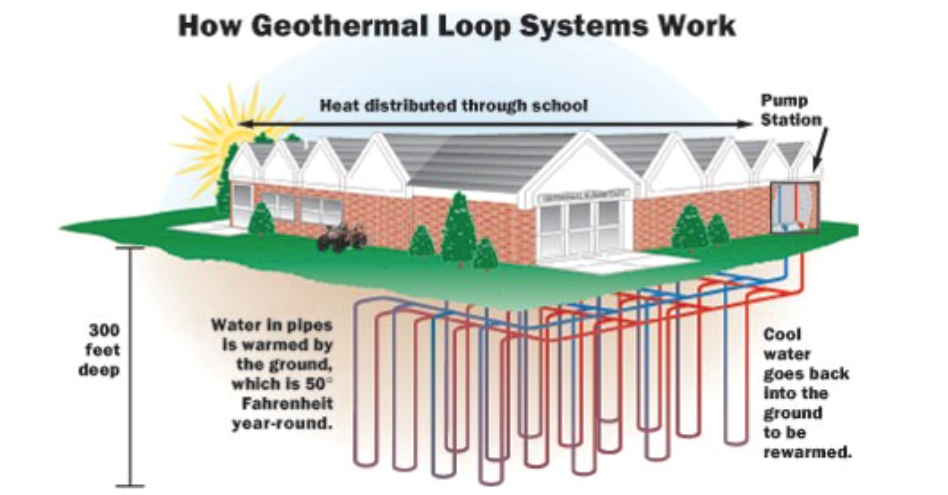
\includegraphics[width=0.9\textwidth]{images/04-GeothermalLoopSystem}
      \caption{Geothermal Loop System (Massachusetts DOER, 2015)}
      \label{fig:geo}
    \end{figure}
    \par The following list shows the advantages and disadvantages of the use and/or installation of Geothermal heating systems. This is a very efficient system but it is important to understand its positive and negative qualities in order to have an efficient system.\\
    
    \vbox{
    \noindent
    Advantages of a Geothermal Heating System:
    \begin{itemize}
      \item{Can provide heating during the winter since the temperature in the Earth will be constant and warmer than the outside air (Massachusetts Department of Energy Resources, 2015).}
      \item{Can provide cooling in the summer by reversing the process and extracting indoor heat from the building and transferring it to the earth through the liquid (Massachusetts Department of Energy Resources, 2015).}
      \item{Lasts for at least 25 years and all the underground components last for more than 50 years (Massachusetts Department of Energy Resources, 2015).}
      \item{A properly installed system can deliver more energy than conventional heating systems, reduce winter costs of heating by half, and heat water for free during the summer (Massachusetts Department of Energy Resources, 2015).}
      \item{There are multiple financing programs and incentives available across the country and especially in Massachusetts through the Department of Energy Resources' programs. (Massachusetts Department of Energy Resources, 2015)}
    \end{itemize}
    }
    \vbox{
    \noindent
    Disadvantages of a Geothermal Heating System:
    \begin{itemize}
      \item{There is a large upfront installation cost associated with geothermal systems (Massachusetts Department of Energy Resources, 2015).}
      \item{Geothermal systems' efficiency can also be very location and geology dependent, which means that in some cases they might not be cost effective (Maehlum, 2014).}
    \end{itemize}
    }

    \subsection{Biomass}
    \par Biomass is a technology that produces energy by burning organic materials. This method is mainly used in buildings to heat the indoor environment or water (Massachusetts Department of Energy Resources, 2015). Figure \ref{fig:bio} is a graphic representation of a wood fueled heating system; in these systems not only logs of wood can be used, but also wood chips and pellets that are more efficient at heating the building and require less storage space (Massachusetts Department of Energy Resources, 2015).
    \begin{figure}[h]
      \centering
        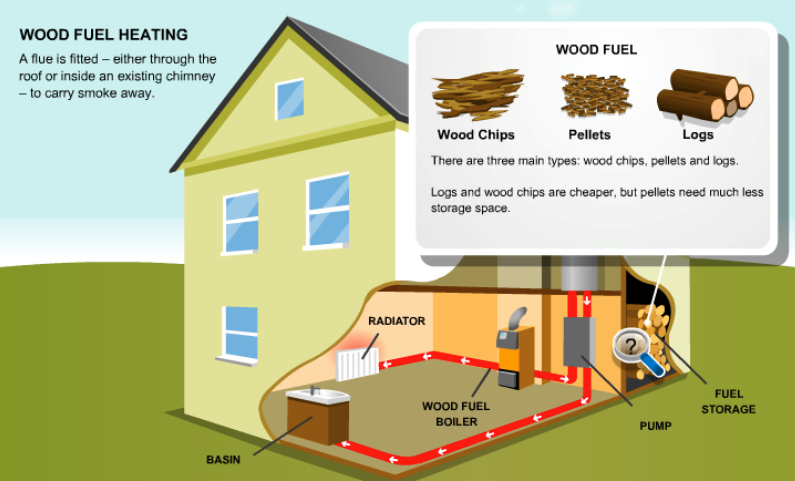
\includegraphics[width=0.75\textwidth]{images/05-BiomassSystem}
      \caption{Biomass System (Massachusetts DOER, 2015)}
      \label{fig:bio}
    \end{figure}
    \par Biomass systems have a variety of positive and negative characteristics related to their use and installation. The following list will mention some advantages and disadvantages of a biomass heating system; this is important in order to understand when the use of this system is most appropriate.\\
    
    \vbox{
    \noindent
    Advantages of a Biomass System:
    \begin{itemize}
      \item{Strengthens the market for locally-sourced energy products, particularly when biomass is produced from waste and residual woods which are byproducts of forestry and manufacturing within the region. This supports the local clean energy economy and job growth (Massachusetts Department of Energy Resources, 2015).}
      \item{Low carbon emission option very suitable for woodlands (Massachusetts Department of Energy Resources, 2015).}
      \item{Most conventional systems are fully automated making them easy to operate and maintain (Massachusetts Department of Energy Resources, 2015).}
      \item{Cost of wood can vary, however it is generally cheaper than the conventional sources of energy such as oil, propane, and electric heat (Massachusetts Department of Energy Resources, 2015).} 
    \end{itemize}
    }
    \vbox{
    \noindent
    Disadvantages of a Biomass System:
    \begin{itemize}
      \item{If used incorrectly it can actually contribute to deforestation (Massachusetts Department of Energy Resources, 2015).}
      \item{It requires a rather large space for storage of the biomass supply. Usually several weeks supply is stored onsite, sometimes in 20-foot tall silos (Massachusetts Department of Energy Resources, 2015).}
      \item{The cost of acquiring a completely new heating system can be higher when compared to conventional fossil fuel heating systems (Massachusetts Department of Energy Resources, 2015).}
    \end{itemize}
    }

    \subsection{Air Source Heat Pumps}
    \par An air source heat pump system consists of an outdoor air compressor/condenser and an indoor air-handling unit. This system is able to heat and cool air by transferring inside and outside air and cooling or heating it through pipes. A mini-split system consists of one air compressor and multiple smaller, indoor air-handling units (Massachusetts Department of Energy Resources, 2015). Figure \ref{fig:ashp} shows how air source heat pump systems function in winter and summer.
    \begin{figure}[h]
      \centering
        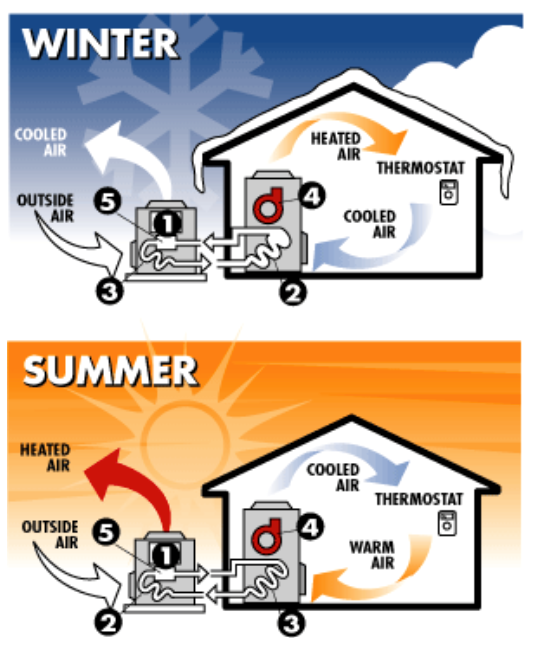
\includegraphics[width=0.5\textwidth]{images/06-AirSourceHeatPump}
      \caption{Air Source Heat Pumps (Massachusetts DOER, 2015)}
      \label{fig:ashp}
    \end{figure}
    \par An Air source heat pump system is a very versatile and affordable system but there are certain conditions that must be met in order to get the most of it and make it efficient, which is why it is important to list the different advantages and disadvantages that this system can have.\\
    
    \vbox{
    \noindent
    Advantages of an Air Source Heat Pump:
    \begin{itemize}
      \item{Can be powered by electricity obtained from solar panels making them energy efficient and clean (Massachusetts Department of Energy Resources, 2015).}
      \item{A ductless mini-split system is a great add-on for non-ducted houses\footnote{Non-ducted houses: Houses that don't have hydronic (hot water heat) systems, radiant panels or space heaters.} (Massachusetts Department of Energy Resources, 2015).}
      \item{Mini-split systems are small and have great flexibility on installation for zoning or heating/cooling individual rooms (Massachusetts Department of Energy Resources, 2015).}
      \item{Low installation cost while still being environmentally friendly (U.S. Department of Energy, 2001)}
    \end{itemize}
    }
    \vbox{
    \noindent
    Disadvantages of an Air Source Heat Pump:
    \begin{itemize}
      \item{Needs regular maintenance (every 2-6 months) including inspecting ducts and lubricating motors (U.S. Department of Energy, 2012).}
      \begin{itemize}
        \item{A severely neglected system will have a lower efficiency by a range of 10-25\%. (U.S. Department of Energy, 2001)}
      \end{itemize}
      \item{There can be many installation and service problems such as leaks in ducts, low airflow, and incorrect refrigerant charge. (U.S. Department of Energy, 2001)}
    \end{itemize}
    }

  \section{Summary}
  \par The industrialized nations' dependence on fossil fuels is unsustainable, damages the environment, and is a threat to public health. Buildings are the largest sector of energy consumption both nationally and in Massachusetts, and heating and cooling account for 50\% of energy consumption within the building energy consumption sector. Consequently, a variety of programs and legislation have been established in Massachusetts that provide funding for and encourage the installation of renewable energy sources to reduce the dependence on fossil fuels. Our sponsor, the Department of Energy Resources, created the DOER Renewable Thermal Program and SAPHIRE, that focus on the installation of renewable thermal heating and cooling systems in different types of buildings. The DOER's renewable thermal programs lack complete narratives explaining the full details and hurdles along the process to implementing a renewable thermal system. This information would allow them to improve their own program and promote further installations of renewable thermal technologies.
